\documentclass[11pt]{article}

\usepackage[letterpaper,left=85pt,right=85pt,top=110pt,bottom=60pt,headheight=86pt,headsep=5pt]{geometry}
\usepackage[spanish,es-noshorthands]{babel}
\usepackage{fontspec}
\usepackage{xcolor}
\usepackage{graphicx}
\usepackage{enumitem}
\usepackage{array}
\usepackage{tabularx}
\usepackage{longtable}
\usepackage{booktabs}
\usepackage{colortbl}
\usepackage{listings}
\usepackage{fancyhdr}
\usepackage{ragged2e}
\usepackage{microtype}
\usepackage{caption}
\usepackage{float}
\usepackage{tikz}
\usepackage{pgfplots}
\pgfplotsset{compat=1.18}
\usetikzlibrary{arrows.meta,positioning,shapes.geometric,fit,calc,backgrounds}
\usepackage[hidelinks]{hyperref}
\usepackage{xurl}

\setlength{\headheight}{86pt}
\setsansfont{Arial}
\newfontfamily\codefont{Consolas}
\renewcommand{\familydefault}{\sfdefault}
\setlength{\parindent}{0pt}
\setlength{\parskip}{8pt}
\linespread{1.0}
\setlength{\emergencystretch}{1.5em}
\setlist[itemize]{leftmargin=1.2em,itemsep=0.05em,topsep=0.10em,parsep=0pt}
\setlist[enumerate]{leftmargin=1.4em,itemsep=0.05em,topsep=0.10em,parsep=0pt}

\definecolor{navy}{HTML}{17324D}
\definecolor{teal}{HTML}{23878A}
\definecolor{gold}{HTML}{D9A441}
\definecolor{coral}{HTML}{CB6651}
\definecolor{mist}{HTML}{E9EEF2}
\definecolor{linegray}{HTML}{B8C1CA}
\definecolor{ink}{HTML}{24303A}
\definecolor{tablehead}{HTML}{E7E6E6}

\hypersetup{hidelinks}

\pagestyle{fancy}
\fancyhf{}
\renewcommand{\headrulewidth}{0pt}
\renewcommand{\footrulewidth}{0pt}
\fancyhead[C]{%
  \raisebox{40pt}[0pt][0pt]{%
    \begin{minipage}{\textwidth}
    \raggedleft
    \fontsize{11}{19}\selectfont\bfseries
    26-AT625\\[-6.3pt]
    ClaudIA: Sistema Inteligente de Acompañamiento Didáctico\\[-1pt]
    para Grupos DGETI
    \end{minipage}%
  }%
}

\renewcommand{\arraystretch}{1.10}
\captionsetup{font=footnotesize,labelfont=bf,labelsep=period,justification=centering,singlelinecheck=false}
\captionsetup[table]{name=Tabla}
\captionsetup[figure]{name=Figura}

\newcommand{\Section}[1]{\par\vspace{0.16\baselineskip}{\normalfont\normalsize\bfseries\RaggedRight #1\par}}
\newcommand{\Subsection}[1]{\par\vspace{0.12\baselineskip}{\normalfont\normalsize\bfseries\RaggedRight #1\par\vspace{0.07\baselineskip}}}
\newcommand{\ManualCaption}[1]{\begin{center}\fontsize{8}{9.5}\selectfont #1\end{center}}
\lstset{
  basicstyle=\codefont\fontsize{7.6}{9.0}\selectfont,
  breaklines=true,
  columns=fullflexible,
  keepspaces=true,
  frame=none,
  aboveskip=0.28\baselineskip,
  belowskip=0.28\baselineskip,
  xleftmargin=0.25in,
  xrightmargin=0.20in
}

\begin{document}
\pagenumbering{gobble}
\fontsize{11}{19}\selectfont

% ---------------------------------------------------------------------------
% INTRODUCCIÓN
% ---------------------------------------------------------------------------
\Section{Introducción}

El acompañamiento didáctico permite que el estudiante transforme una consigna en acciones, reconozca sus errores y solicite ayuda antes de abandonar la tarea. Su valor depende de que la orientación llegue cuando aparece la duda y de que el alumno conserve la responsabilidad de elaborar la respuesta.

ClaudIA propone una estación física de apoyo dentro del aula. El estudiante habla, escucha una explicación breve y continúa con preguntas o ejemplos. No necesita instalar una aplicación ni trasladar la conversación a otro dispositivo. Mientras tanto, el docente recibe información agregada sobre los temas que requieren intervención.

La estación no entrega la respuesta final: conduce al estudiante mediante intentos, pistas y preguntas de comprobación. Su presencia física busca familiaridad y acceso compartido, pero exige señalización visible y reglas claras para el uso de micrófono y cámara.

El proyecto se alinea con el MCCEMS, que promueve respuestas a contextos locales y una formación humanista e integral \cite{sep2025mccms}, y con la línea de desarrollo tecnológico del PROIDET \cite{dgeti2026}.

\clearpage

% ---------------------------------------------------------------------------
% PÁGINA 5 - PROBLEMA
% ---------------------------------------------------------------------------
\Section{Planteamiento del problema}

En la muestra diagnosticada, las dificultades académicas aparecen como problemas de organización, comprensión y administración del tiempo. Se relacionan entre sí: una consigna mal interpretada puede retrasar la tarea, una fecha olvidada acumula pendientes y una duda no expresada llega al docente cuando el rezago ya se consolidó.

La limitación principal es de atención. El docente puede explicar para el grupo, pero no observar al mismo tiempo cada intento, corregir todos los errores y registrar qué concepto genera más dificultad. Las plataformas convencionales añaden pasos de acceso; ClaudIA reduce esa fricción mediante una pregunta oral y una conversación guiada.

El problema central es la ausencia de un apoyo pedagógico permanente y accesible que convierta el trabajo cotidiano del aula en explicación, práctica y retroalimentación, sin operar como vigilancia ni como sustituto docente.

En México, INEGI e IFT reportan que 86.1\% de la población de seis años o más usó internet en 2025 y que 97.0\% de las personas usuarias de telefonía móvil tenía un teléfono inteligente \cite{inegi2026}. La cobertura es amplia, aunque persisten brechas urbano-rurales; por ello, ClaudIA debe tolerar conectividad limitada.

Licona advierte que la IA puede ampliar el acceso educativo y, a la vez, profundizar exclusiones si faltan alfabetización, infraestructura y formación docente \cite{licona2024}. El diseño debe ser complementario, verificable y capaz de operar sin servicios remotos.

\clearpage

% ---------------------------------------------------------------------------
% PÁGINA 6 - JUSTIFICACIÓN
% ---------------------------------------------------------------------------
\Section{Justificación}

La necesidad observada justifica una ayuda inmediata que no se limite a responder. ClaudIA puede solicitar un razonamiento, ofrecer una pista, comprobar el avance y proponer otra variante; así se aproxima a la tutoría y se aleja del simple buscador.

El meta-análisis de Ma, Adesope, Nesbit y Liu encontró un tamaño de efecto de $g=0.57$ a favor de sistemas de tutoría inteligente frente a instrucción computarizada sin tutoría, y de $g=0.42$ frente a la enseñanza en grupos grandes \cite{ma2014}. El resultado respalda el potencial de esta mediación, pero también exige un diseño pedagógico riguroso.

Gubareva y Lopes muestran que los asistentes virtuales ayudan a organizar el estudio, administrar el tiempo y sostener la motivación cuando el apoyo individual resulta costoso \cite{gubareva2020}. ClaudIA traslada esa función a una estación compartida y la concentra en la conversación oral.

La UNESCO advierte que una respuesta fluida puede ser incorrecta. Por ello, la supervisión humana, la verificación y la transparencia son condiciones de uso de la IA generativa \cite{unesco2024guide}; ClaudIA no aceptará una explicación sólo porque provenga de un modelo.

\clearpage

% ---------------------------------------------------------------------------
% PÁGINA 7 - PROPÓSITO Y OBJETIVOS
% ---------------------------------------------------------------------------
\Section{Propósito, hipótesis y objetivos}

\Subsection{Hipótesis de trabajo}
La mediación oral y dialógica de ClaudIA permitirá que estudiantes de un grupo DGETI obtengan apoyo oportuno para organizar actividades y comprender temas, y que el docente identifique con mayor rapidez los contenidos que requieren nueva explicación. La hipótesis se evaluará con un piloto dentro del plantel y no se asume como resultado ya demostrado.

\Subsection{Objetivo general}
Desarrollar una estación modular de acompañamiento didáctico que integre escucha, respuesta hablada, percepción de presencia y seguimiento pedagógico para apoyar el trabajo de estudiantes y docentes en grupos de Educación Media Superior.

\Subsection{Objetivos específicos}
\begin{enumerate}
  \item Identificar las necesidades académicas y prácticas de uso de IA de estudiantes del CETis 20.
  \item Adaptar una base tecnológica modular existente a la identidad, configuración y experiencia de ClaudIA.
  \item Integrar entrada de voz, salida por bocina y detección de presencia o entorno.
  \item Diseñar flujos de explicación, pregunta guiada, práctica y retroalimentación formativa.
  \item Mantener contexto de la clase y progreso de práctica sin conservar datos innecesarios.
  \item Proporcionar al docente un resumen agregado de dudas y temas que requieren apoyo.
  \item Evaluar claridad, utilidad, accesibilidad, estabilidad y aceptación durante un piloto escolar.
\end{enumerate}

\Subsection{Límites del proyecto}
ClaudIA no emite diagnósticos médicos o psicológicos, no califica automáticamente una asignatura y no sustituye la asesoría docente. La cámara se destina a detectar presencia o contexto general del entorno; no identifica estudiantes, no reconoce rostros y no procesa cuadernos para resolver ejercicios. El dispositivo no aprende de conversaciones sin una regla explícita y auditable.

\clearpage

% ---------------------------------------------------------------------------
% PÁGINA 8 - METODOLOGÍA
% ---------------------------------------------------------------------------
\Section{Metodología}

El proyecto combina investigación aplicada, diseño de prototipo y evaluación formativa. La fase diagnóstica es exploratoria y descriptiva; reúne 122 registros de estudiantes del CETis 20 para identificar dificultades académicas y prácticas de uso y verificación de IA.

\Subsection{Diseño muestral}
Muestra de conveniencia con 122 registros únicos del plantel participante. Los porcentajes se calcularon sobre el total de respuestas y se usan para formular requisitos de diseño.

\Subsection{Procesamiento estadístico}
Se obtuvieron distribuciones de frecuencia y porcentajes sobre el conjunto total. No se aplicaron pruebas inferenciales porque la muestra no es probabilística; los resultados constituyen una línea base y no permiten afirmar efectos causales.

\Subsection{Diseño tecnológico}
La construcción parte de una arquitectura modular ya operativa y añade adaptadores para la estación física. La validación actual es técnica y automatizada; la validación educativa corresponde al piloto.

\clearpage

% ---------------------------------------------------------------------------
% PÁGINA 9 - MUESTRA AGREGADA
% ---------------------------------------------------------------------------
\Section{Muestra total del CETis 20}

La base analizada contiene 122 respuestas únicas de estudiantes del CETis 20. El análisis no presenta desgloses internos del alumnado: todos los resultados se interpretan sobre el mismo total y cada porcentaje utiliza un denominador de 122 casos.

\begin{table}[H]
\centering
\caption{Ficha agregada de la muestra}
\begin{tabular}{lr}
\toprule
\textbf{Indicador} & \textbf{Valor} \\
\midrule
Plantel & CETis 20 \\
Respuestas analizadas & 122 \\
Identificadores únicos & 122 \\
Registro de campo & 26 y 27 de octubre de 2026 \\
Diseño & Muestra de conveniencia \\
Uso & Requisitos y línea base \\
\bottomrule
\end{tabular}
\end{table}

La revisión de calidad confirmó que los 122 identificadores son diferentes y que las variables analizadas no contienen valores faltantes.

La selección fue intencional y no probabilística. Por ello, los porcentajes describen al conjunto participante del CETis 20 y no se extrapolan como estimaciones de todo el plantel.

\clearpage

% ---------------------------------------------------------------------------
% PÁGINA 10 - NECESIDADES
% ---------------------------------------------------------------------------
\Section{Necesidades académicas}

Organizarse o recordar fechas fue la dificultad principal para 46 estudiantes; entender el tema, para 45. Juntas concentran 74.6\% de las respuestas. La falta de tiempo aparece en tercer lugar, con 30 casos, y sólo una persona eligió el acceso a internet o dispositivo.

\begin{figure}[H]
\centering
\resizebox{0.98\textwidth}{!}{%
\begin{tikzpicture}
\begin{axis}[
  width=0.9\textwidth,
  height=6.4cm,
  xbar,
  xmin=0,
  xmax=58,
  symbolic y coords={Internet o dispositivo,Falta de tiempo,Entender el tema,Organizarme o recordar fechas},
  y dir=reverse,
  title={Dificultad académica principal},
  title style={align=left,font=\bfseries\color{navy}},
  xlabel={Número de estudiantes},
  axis x line*=bottom,
  axis y line*=left,
  tick label style={font=\small},
  axis line style={draw=linegray},
  xmajorgrids,
  grid style={draw=mist},
  nodes near coords,
  nodes near coords style={font=\scriptsize,color=navy},
  bar width=13pt,
  fill=coral,
  draw=none
]
\addplot coordinates {
  (1,Internet o dispositivo)
  (30,Falta de tiempo)
  (45,Entender el tema)
  (46,Organizarme o recordar fechas)
};
\end{axis}
\end{tikzpicture}
}
\caption{Respuesta única sobre la principal dificultad, $n=122$.}
\end{figure}

Estos datos orientan tres funciones: dividir una meta amplia en acciones breves, apoyar la recuperación de entregas y detectar el punto donde se interrumpe la comprensión. Responder preguntas no basta; la estación también debe enseñar a planear, revisar y corregir.

\clearpage

% ---------------------------------------------------------------------------
% RELACIÓN DE LOS ESTUDIANTES CON LA IA
% ---------------------------------------------------------------------------
\Section{Relación de los estudiantes con la IA}

La familiaridad con la IA es alta: 59.8\% usa una respuesta si le parece correcta, 32.8\% verifica con fuentes o con el docente y 7.4\% no la utiliza. La diferencia muestra que el acceso ya existe, pero la verificación sistemática todavía es limitada.

\begin{figure}[H]
\centering
\resizebox{0.98\textwidth}{!}{%
\begin{tikzpicture}
\begin{axis}[
  width=0.93\textwidth,
  height=6.2cm,
  xbar,
  xmin=0,
  xmax=88,
  symbolic y coords={No uso IA,Verifico con fuentes o docente,La uso si parece correcta},
  y dir=reverse,
  title={Forma de uso declarada de la IA},
  title style={align=left,font=\bfseries\color{navy}},
  xlabel={Número de estudiantes},
  axis x line*=bottom,
  axis y line*=left,
  tick label style={font=\small},
  axis line style={draw=linegray},
  xmajorgrids,
  grid style={draw=mist},
  nodes near coords,
  nodes near coords style={font=\scriptsize,color=navy},
  bar width=16pt,
  fill=gold,
  draw=none
]
\addplot coordinates {
  (9,No uso IA)
  (40,Verifico con fuentes o docente)
  (73,La uso si parece correcta)
};
\end{axis}
\end{tikzpicture}
}
\caption{Uso y verificación declarados de IA, $n=122$.}
\end{figure}

La UNESCO propone una competencia en IA centrada en las personas, la ética y el diseño de sistemas \cite{miao2024}, y advierte que la fluidez de un modelo no garantiza exactitud \cite{unesco2024guide}. ClaudIA debe solicitar intentos, pedir justificación y derivar al docente cuando no tenga evidencia suficiente.

\Subsection{Alcance de los datos}
La encuesta describe hábitos y necesidades, pero no demuestra aceptación de la estación ni mejoras de aprendizaje. Esos efectos deberán medirse en el piloto.

\clearpage

% ---------------------------------------------------------------------------
% LÍMITES DE LA EVIDENCIA
% ---------------------------------------------------------------------------
\Section{Límites de la evidencia y validación necesaria}

La encuesta justifica la necesidad y muestra familiaridad con la IA; no permite inferir mejoras de aprendizaje, aceptación de la voz o tolerancia a la cámara. La siguiente etapa debe observar esos aspectos en condiciones reales.

\Subsection{Aspectos que necesitan medición}
Antes de medir efectos educativos se requiere comprobar aceptación, usabilidad y confianza institucional.

\begin{table}[H]
\centering
\caption{Preguntas específicas para la siguiente validación}
\footnotesize
\begin{tabularx}{\textwidth}{@{}>{\raggedright\arraybackslash}p{1.28in}>{\raggedright\arraybackslash}X@{}}
\toprule
\textbf{Dimensión} & \textbf{Pregunta propuesta} \\
\midrule
Interacción oral & ¿Qué tan cómodo te resultaría preguntar en voz alta a ClaudIA dentro del aula? \\
Pedagogía & Cuando no comprendes un tema, ¿prefieres un ejemplo, una pista, una pregunta guía o una explicación más breve? \\
Verificación & ¿Qué haría que confiaras o desconfiaras de una explicación dada por ClaudIA? \\
Presencia & ¿Cómo te sientes al saber que la cámara sólo detecta que hay personas frente a la estación y no identifica rostros? \\
Privacidad & ¿Qué información de tu participación no debería guardar el sistema? \\
Docente & ¿Qué resumen sería útil para decidir una nueva explicación sin observar conversaciones completas? \\
\bottomrule
\end{tabularx}
\end{table}

\Subsection{Diseño de la interacción}
El diálogo se organizará como una ayuda gradual:
\begin{enumerate}
  \item ClaudIA escucha la duda y confirma lo que entendió.
  \item Pide al estudiante que explique qué sabe o qué intentó.
  \item Ofrece un ejemplo análogo, no el resultado del ejercicio.
  \item Formula una pregunta que haga visible el siguiente paso.
  \item Solicita un nuevo intento o, si persiste el bloqueo, deriva al docente.
\end{enumerate}

\clearpage

% ---------------------------------------------------------------------------
% PÁGINA 13 - REQUISITOS DE DISEÑO
% ---------------------------------------------------------------------------
\Section{Requisitos de diseño derivados de la evidencia}

Los datos no justifican otro chatbot genérico. Orientan una estación que combine organización del trabajo, explicación y práctica. La tabla relaciona cada hallazgo con una decisión de diseño.

\begin{table}[H]
\centering
\caption{Relación entre diagnóstico y diseño de ClaudIA}
\small
\begin{tabularx}{\textwidth}{@{}>{\raggedright\arraybackslash}p{1.42in}>{\raggedright\arraybackslash}X>{\raggedright\arraybackslash}p{1.55in}@{}}
\toprule
\textbf{Evidencia} & \textbf{Necesidad} & \textbf{Función} \\
\midrule
37.7\% dificultad para organizarse & Dividir metas y recordar fechas & Plan de sesión y recordatorio contextual \\
36.9\% dificultad para entender & Explicación gradual con ejemplos & Tutor oral paso a paso \\
24.6\% falta de tiempo & Interacciones breves y recuperables & Micropíldoras de 3 a 7 minutos \\
92.6\% usa IA & Aprovechar familiaridad & Lenguaje natural y práctica guiada \\
32.8\% verifica con fuentes & Evitar dependencia & Comprobación y derivación al docente \\
\bottomrule
\end{tabularx}
\end{table}

\Subsection{Decisión central}
El micrófono y la cámara sólo aportan información de entrada. La respuesta pedagógica se construye con preguntas, ejemplos, explicaciones breves y pistas; la resolución automática queda fuera del alcance.

\clearpage

% ---------------------------------------------------------------------------
% PÁGINA 14 - MARCO PEDAGÓGICO
% ---------------------------------------------------------------------------
\Section{Marco pedagógico}

\Subsection{Aprendizaje autorregulado}
La Education Endowment Foundation (EEF), fundación británica dedicada a generar y sintetizar evidencia sobre prácticas educativas, describe al estudiante autorregulado como alguien que conoce sus fortalezas y debilidades y puede planear, monitorear y evaluar su aprendizaje. En estudiantes novatos, esas estrategias deben hacerse explícitas \cite{eef2018}. ClaudIA puede convertir cada interacción en una pequeña estructura de autorregulación:
\begin{enumerate}
  \item \textbf{Planear:} ``¿Qué tienes que resolver y qué sabes ya?''
  \item \textbf{Monitorear:} ``¿En qué paso apareció la duda?''
  \item \textbf{Evaluar:} ``¿Cómo sabes que tu respuesta es razonable?''
\end{enumerate}

\Subsection{Retroalimentación formativa}
La EEF recomienda que la retroalimentación se base en una instrucción de calidad, esté oportunamente ubicada y se dirija hacia la tarea, el contenido y las estrategias de autorregulación. La retroalimentación vaga o centrada en rasgos personales suele ser menos eficaz \cite{eef2021}. Por eso, ClaudIA no dirá simplemente ``eres bueno en matemáticas''. Dirá qué parte del procedimiento está bien, qué paso debe revisar y qué pregunta puede probar.

\Subsection{Tutoría con pistas}
La tutoría convierte la ayuda en práctica guiada: comprender el objetivo, pedir un intento, ubicar el error, ofrecer una pista, permitir otro intento y comparar el razonamiento con un caso parecido.

\Subsection{Enseñanza situada}
El apoyo toma ejemplos del contexto y del material que el docente está trabajando. La base educativa actual ya contiene lecciones, objetivos, pasos y ejercicios breves; ClaudIA ampliará ese catálogo con contenidos de las asignaturas del plantel.

\clearpage

% ---------------------------------------------------------------------------
% PÁGINA 15 - VOZ, VISIÓN Y ACCESIBILIDAD
% ---------------------------------------------------------------------------
\Section{Interfaz oral, percepción y accesibilidad}

\Subsection{Entrada por voz}
La voz reduce la fricción de escribir en un dispositivo compartido. El estudiante puede formular una duda mientras tiene el cuaderno en las manos. Sin embargo, el reconocimiento puede fallar por ruido de aula, acento o vocabulario técnico. ClaudIA debe confirmar verbalmente lo que entendió, pedir repetición cuando sea necesario y permitir una corrección oral.

\Subsection{Percepción por cámara}
La cámara aporta una señal de presencia o contexto para activar, pausar o ajustar la estación. Su uso no convierte imágenes de cuadernos, gestos o rostros en información académica.

\Subsection{Diseño universal}
CAST propone diversificar la representación, la acción y la expresión, y el compromiso \cite{cast2024}. ClaudIA aplicará ese principio con explicaciones en distintos niveles, ejemplos, analogías, ritmo ajustable y una opción para repetir. La voz será el canal principal de participación; la cámara no sustituye la expresión del estudiante.

\begin{table}[H]
\centering
\caption{Principios de accesibilidad aplicados al dispositivo}
\begin{tabularx}{\textwidth}{@{}lX@{}}
\toprule
\textbf{Principio} & \textbf{Aplicación concreta} \\
\midrule
Múltiples formas de representación & Ejemplos, analogías, resúmenes breves y repetición oral \\
Múltiples formas de acción & Formular una duda, explicar con palabras propias o pedir una pista \\
Múltiples formas de participación & Práctica corta, retos por niveles y pista antes de respuesta \\
\bottomrule
\end{tabularx}
\end{table}

\clearpage

% ---------------------------------------------------------------------------
% PÁGINA 16 - ÉTICA Y PRIVACIDAD
% ---------------------------------------------------------------------------
\Section{Ética, privacidad y control}

La cámara y el micrófono modifican el nivel de riesgo frente a un chatbot de texto. NIST propone un ciclo de gobernar, mapear, medir y gestionar los riesgos de IA \cite{nist2023}; su perfil de IA generativa añade riesgos de confiabilidad, privacidad, sesgo e información incorrecta \cite{nist2024}. Una revisión sobre cámaras en escuelas advierte que la vigilancia continua puede erosionar autonomía y privacidad cuando no existen límites explícitos \cite{zulfiqar2026}.

ClaudIA responderá con siete controles:
\begin{enumerate}
  \item \textbf{Detección deliberada:} la cámara sólo detecta presencia o contexto y se desactiva cuando no hay una sesión autorizada.
  \item \textbf{Sin reconocimiento facial:} el sistema no identifica estudiantes ni infiere emociones.
  \item \textbf{Indicador físico:} luz y obturador muestran cuándo la cámara está activa.
  \item \textbf{Minimización:} se conserva la transcripción educativa necesaria, no el audio ni el video completos.
  \item \textbf{Retención limitada:} los datos de práctica se eliminan o anonimizan al terminar el periodo definido.
  \item \textbf{Acceso por roles:} estudiantes, docentes y administradores tienen permisos distintos.
  \item \textbf{Supervisión humana:} una alerta sugiere revisión; no determina sanciones ni calificaciones.
\end{enumerate}

\Subsection{Uso responsable de IA}
La UNESCO promueve un enfoque centrado en las personas, con protección de la privacidad y participación humana \cite{unesco2024guide}. ClaudIA mostrará cuándo una respuesta proviene de un modelo, permitirá corregir una transcripción, rechazará contenidos fuera del contexto escolar y pedirá ayuda docente cuando no tenga evidencia suficiente.

\clearpage

% ---------------------------------------------------------------------------
% PÁGINA 17 - PRESENTACIÓN DE CLAUDIA
% ---------------------------------------------------------------------------
\Section{Presentación de ClaudIA}

ClaudIA será una estación de acompañamiento con cuatro componentes visibles: una carcasa estable, un micrófono, una bocina y una cámara con protector. Un procesador local ejecuta el núcleo y coordina las integraciones. La estación puede operar conectada a la red del plantel y usar servicios de IA cuando estén disponibles.

\begin{center}
\resizebox{0.98\textwidth}{!}{%
\begin{tikzpicture}[
  node distance=8mm,
  box/.style={draw=linegray,rounded corners=4pt,fill=white,minimum height=0.8cm,align=center,font=\small},
  accent/.style={draw=teal,rounded corners=4pt,fill=teal!8,minimum height=0.9cm,align=center,font=\small\bfseries},
  arrow/.style={-{Stealth[length=2.4mm]},draw=linegray,line width=0.7pt}
]
\node[accent,text width=2.1cm] (student) {Estudiante};
\node[box,right=of student,text width=2.35cm] (mic) {Micrófono\\voz};
\node[box,right=of mic,text width=2.4cm] (core) {Núcleo ClaudIA\\intención y contexto};
\node[box,right=of core,text width=2.45cm] (tutor) {Tutor y lógica\\pedagógica};
\node[box,right=of tutor,text width=2.3cm] (speaker) {Bocina\\respuesta oral};
\draw[arrow] (student) -- (mic);
\draw[arrow] (mic) -- (core);
\draw[arrow] (core) -- (tutor);
\draw[arrow] (tutor) -- (speaker);
\draw[arrow,bend left=18] (speaker) to node[below,font=\scriptsize,text=linegray]{retroalimentación} (student);

\node[box,below=of core,text width=2.35cm] (camera) {Cámara\\presencia};
\node[box,below=of tutor,text width=2.35cm] (vision) {Percepción\\personas y entorno};
\node[box,below=of speaker,text width=2.25cm] (teacher) {Docente\\panel resumido};
\draw[arrow] (camera) -- node[left,font=\scriptsize]{presencia} (core);
\draw[arrow] (camera) -- (vision);
\draw[arrow] (vision) -- (core);
\draw[arrow] (tutor) -- node[right,font=\scriptsize]{alertas} (teacher);
\end{tikzpicture}
}
\end{center}

\begin{table}[H]
\centering
\caption{Casos de uso principales}
\begin{tabularx}{\textwidth}{@{}>{\raggedright\arraybackslash\bfseries}p{1.65in}X@{}}
\toprule
Acción & Resultado pedagógico \\
\midrule
``Explícame este paso'' & Explicación oral breve, ejemplo y comprobación \\
``Dame una pista'' & Pregunta guía y avance sin revelar la solución \\
``¿Cuál es la respuesta?'' & Pide un intento o reformula el razonamiento; no expone el resultado \\
``Hazme una pregunta'' & Práctica activa con retroalimentación \\
``¿Qué vimos hoy?'' & Recuperación del contexto de la sesión \\
``No entendí'' & Reformulación con otro ejemplo o derivación al docente \\
\bottomrule
\end{tabularx}
\end{table}

\clearpage

% ---------------------------------------------------------------------------
% PÁGINA 18 - ARQUITECTURA
% ---------------------------------------------------------------------------
\Section{Arquitectura del sistema}

La arquitectura conserva la separación del código base: las interfaces no llaman directamente al modelo; los comandos no contienen reglas pedagógicas; la memoria temporal no se mezcla con el progreso educativo. Esta división permite sustituir micrófono, cámara o proveedor de IA sin reescribir el núcleo.

\begin{center}
\resizebox{0.66\textwidth}{!}{%
\begin{tikzpicture}[
  node distance=7mm and 8mm,
  layer/.style={draw=linegray,rounded corners=5pt,minimum width=3.4cm,minimum height=0.9cm,align=center,font=\small},
  hw/.style={layer,fill=gold!15},
  iface/.style={layer,fill=teal!12},
  core/.style={layer,fill=navy!10},
  data/.style={layer,fill=coral!10}
]
\node[hw] (hardware) {Hardware\\micrófono, cámara, bocina};
\node[iface,below=of hardware] (adapter) {Adaptadores\\audio y presencia};
\node[core,below=of adapter] (eventbus) {Núcleo y eventos\\estado y ruteo};
\node[core,below=of eventbus] (intent) {Comandos / intención\\sesiones y reglas};
\node[core,below=of intent] (edu) {Tutor + educación\\lecciones y ejercicios};
\node[data,right=of eventbus] (memory) {Memoria\\sesión y progreso};
\node[data,right=of edu] (ai) {Servicio IA\\respuesta contextual};
\node[data,right=of intent] (logs) {Registro\\evidencia mínima};
\draw[-{Stealth},draw=linegray] (hardware)--(adapter);
\draw[-{Stealth},draw=linegray] (adapter)--(eventbus);
\draw[-{Stealth},draw=linegray] (eventbus)--(intent);
\draw[-{Stealth},draw=linegray] (intent)--(edu);
\draw[<->,draw=linegray] (eventbus)--(memory);
\draw[<->,draw=linegray] (edu)--(ai);
\draw[-{Stealth},draw=linegray] (intent)--(logs);
\end{tikzpicture}
}
\end{center}

\Subsection{Flujo de una consulta}
El micrófono produce texto; el adaptador normaliza la entrada y emite un evento. El núcleo identifica si se trata de un comando, una duda o una solicitud de práctica. El módulo educativo recupera lección, contexto y progreso. Si la consulta requiere explicación adaptativa, se consulta el servicio de IA con límites de seguridad. La respuesta se convierte en audio y, cuando corresponde, se resume para el docente.

La cámara sigue un flujo independiente. Detecta si hay una persona frente a la estación y obtiene una señal general del entorno para activar, pausar o ajustar la interacción. No interpreta el contenido de un cuaderno ni convierte una imagen en una pregunta académica. El video no se conserva.

\clearpage

% ---------------------------------------------------------------------------
% PÁGINA 19 - EXPERIENCIA DEL ESTUDIANTE
% ---------------------------------------------------------------------------
\Section{Experiencia del estudiante}

La interacción debe sentirse como una consulta de aula, no como una prueba de vigilancia. El estudiante se acerca, activa la sesión con una frase o botón, pregunta y recibe una respuesta. El dispositivo debe indicar de forma perceptible cuándo escucha y cuándo observa.

\Subsection{Recorrido de uso}
\begin{enumerate}
  \item \textbf{Activación:} ``ClaudIA, necesito ayuda con esta ecuación''.
  \item \textbf{Confirmación:} la estación repite oralmente lo que entendió.
  \item \textbf{Contexto:} pregunta qué intentó y qué parte no comprende.
  \item \textbf{Diagnóstico:} identifica el paso donde se produjo el bloqueo.
  \item \textbf{Pista:} ofrece una pregunta o regla, sin resolver el ejercicio.
  \item \textbf{Intento:} el estudiante explica o resuelve de nuevo.
  \item \textbf{Cierre:} pide una explicación final y registra sólo el tema y el avance.
\end{enumerate}

\Subsection{Ejemplo de diálogo}
\begin{quote}
\small
\textbf{Estudiante:} No entiendo por qué la derivada de $x^2$ es $2x$.\\
\textbf{ClaudIA:} Vamos a verlo con una pregunta. Si $y=x^2$, ¿qué significa el exponente 2?\\
\textbf{Estudiante:} Que se multiplica $x$ por $x$.\\
\textbf{ClaudIA:} Correcto. Ahora piensa qué ocurre cuando cambia el valor de $x$. ¿Qué relación observas entre el exponente original y el nuevo factor?\\
\textbf{Estudiante:} Queda $x^1$ y adelante un 2.\\
\textbf{ClaudIA:} Ese paso es consistente. Antes de continuar, explica con tus palabras por qué aparece ese factor y prueba con otro exponente.
\end{quote}

\Subsection{Reglas de interacción}
La sesión puede pausarse o cerrarse en cualquier momento. Si la transcripción no es confiable, ClaudIA pide repetición; al finalizar, el estudiante puede borrar el contexto temporal sin eliminar el progreso pedagógico autorizado.

\clearpage

% ---------------------------------------------------------------------------
% PÁGINA 20 - DOCENTE
% ---------------------------------------------------------------------------
\Section{Apoyo al docente}

El docente no necesita revisar cada conversación. ClaudIA presenta un resumen de patrones: temas consultados, tipos de error, estudiantes que requirieron apoyo adicional y actividades que quedaron incompletas. La información se agrega por grupo y se muestra con un identificador seudónimo. La identidad se vincula únicamente cuando existe una necesidad pedagógica autorizada.

\begin{table}[H]
\centering
\caption{Vista propuesta para el panel docente}
\begin{tabularx}{\textwidth}{@{}>{\raggedright\arraybackslash}p{1.36in}>{\raggedright\arraybackslash}X>{\centering\arraybackslash}p{0.9in}@{}}
\toprule
\textbf{Indicador} & \textbf{Qué muestra} & \textbf{Frecuencia} \\
\midrule
Temas consultados & Conceptos que generaron más solicitudes & Diaria \\
Errores frecuentes & Pasos o procedimientos con mayor dificultad & Semanal \\
Prácticas completadas & Ejercicios finalizados por el grupo & Diaria \\
Necesidad de nueva explicación & Contenidos con pistas repetidas o abandono & Semanal \\
Sesiones asistidas & Uso de ClaudIA por sesión o grupo & Diaria \\
\bottomrule
\end{tabularx}
\end{table}

La alerta no etiqueta al estudiante ni predice reprobación. Señala la necesidad de revisar el trabajo, formular una pregunta al grupo o proponer otra actividad; la intervención sigue siendo decisión del docente.

\Subsection{Controles para el aula}
\begin{itemize}
  \item Inicio de sesión del docente con permisos de revisión.
  \item Modo clase para proyectar una pregunta común.
  \item Botón de pausa para que la estación deje de escuchar.
  \item Exportación de un resumen sin audio ni video.
  \item Registro de cambios y consultas de datos para auditoría.
\end{itemize}

\clearpage

% ---------------------------------------------------------------------------
% PÁGINA 21 - HARDWARE
% ---------------------------------------------------------------------------
\Section{Diseño físico propuesto}

La estación puede construirse a partir de una computadora compacta, una cámara USB con obturador, un micrófono de escritorio o arreglo y una bocina amplificada. La carcasa debe estabilizar los componentes, facilitar el acceso a puertos y proteger la ventilación. No se requiere un robot móvil para cumplir el objetivo pedagógico.

\begin{table}[H]
\centering
\caption{Componentes de la estación ClaudIA}
\begin{tabularx}{\textwidth}{@{}>{\bfseries}p{1.35in}X>{\raggedright\arraybackslash}p{1.2in}@{}}
\toprule
Componente & Función & Estado \\
\midrule
Micrófono & Captura de voz y transcripción & Integración web inicial \\
Bocina & Lectura de respuestas, pistas y avisos & Síntesis del navegador \\
Cámara & Detección de presencia y contexto general & Base técnica parcial \\
Unidad de cómputo & Núcleo, módulos y almacenamiento local & Base funcional \\
Carcasa & Estabilidad, señalización y protección & Por fabricar \\
Conectividad & Servicios de IA y sincronización & Por validar en aula \\
\bottomrule
\end{tabularx}
\end{table}

\Subsection{Condiciones de instalación}
La estación debe ubicarse en un punto visible, con alimentación protegida, cableado fuera de zonas de paso y acceso supervisado. El micrófono requiere una distancia que evite captar toda la conversación; la cámara se orienta sólo a la zona de interacción.

\Subsection{Operación mínima}
\begin{itemize}
  \item Botón o palabra de activación.
  \item Indicador de escucha y de cámara activa.
  \item Confirmación oral de las transcripciones.
  \item Respuesta hablada a través de la bocina.
  \item Modo de baja conectividad con actividades precargadas.
  \item Reinicio seguro sin pérdida del progreso registrado.
\end{itemize}

\clearpage

% ---------------------------------------------------------------------------
% PÁGINA 22 - DESARROLLO E INTEGRACIÓN
% ---------------------------------------------------------------------------
\Section{Desarrollo e integración del sistema}

La base tecnológica de ClaudIA es una arquitectura modular que integra núcleo conversacional, bus de eventos, comandos, sesión, memoria persistente, catálogo de lecciones, progreso educativo, lectura de documentos, voz web y visión. El repositorio verificado en el commit \texttt{29db70a} reportó 92 pruebas aprobadas y cero fallos.

\begin{table}[H]
\centering
\caption{Estado de los componentes del sistema}
\small
\begin{tabularx}{\textwidth}{@{}>{\raggedright\arraybackslash}p{1.55in}>{\raggedright\arraybackslash}X>{\centering\arraybackslash}p{0.85in}@{}}
\toprule
\textbf{Módulo} & \textbf{Función aprovechable} & \textbf{Estado} \\
\midrule
Núcleo y eventos & Recibir, enrutar y responder & Funcional \\
Comandos & Separar intención y ejecución & Funcional \\
Memoria y sesión & Mantener contexto y progreso & Funcional \\
Educación & Lecciones, metas y estado & Funcional base \\
Tutor & Explicar, practicar y dar pistas & Funcional base \\
Documentos & Cargar textos de apoyo & Funcional TXT/MD \\
Voz web & Micrófono y síntesis & Funcional en navegador \\
Visión & Detección de presencia y puente Python & Base parcial \\
\bottomrule
\end{tabularx}
\end{table}

La consolidación de ClaudIA requiere cinco acciones principales:
\begin{enumerate}
  \item completar la identidad y los textos visibles;
  \item consolidar la sesión de aula con roles diferenciados;
  \item integrar la detección de presencia sin identificar personas;
  \item incorporar audio físico y un indicador de estado;
  \item construir el panel docente y la política de retención.
\end{enumerate}

Estas acciones preservan la arquitectura. La integración se realizará por módulos y con pruebas de regresión para mantener estables la memoria, el tutor y la interacción por voz.

\clearpage

% ---------------------------------------------------------------------------
% PÁGINA 23 - EVALUACIÓN
% ---------------------------------------------------------------------------
\Section{Plan de evaluación y nivel de madurez}

El piloto se realizará en el CETis 20 con una medición inicial de organización, comprensión y disposición de uso. Después se observarán sesiones guiadas y se evaluarán claridad, utilidad, accesibilidad, privacidad y estabilidad.

\begin{table}[H]
\centering
\caption{Indicadores del piloto}
\begin{tabularx}{\textwidth}{@{}>{\raggedright\arraybackslash}p{1.75in}>{\raggedright\arraybackslash}X@{}}
\toprule
\textbf{Dimensión} & \textbf{Medida propuesta} \\
\midrule
Organización & Actividades registradas y completadas dentro del plazo \\
Comprensión & Preguntas de práctica resueltas después de una pista \\
Autonomía & Número de intentos antes de solicitar la solución \\
Accesibilidad & Estudiantes que completan la interacción exclusivamente por voz \\
Uso del docente & Temas agregados que generan nueva explicación \\
Privacidad & Detección visible y sin conservación de video \\
Estabilidad & Errores técnicos, interrupciones y recuperación de sesión \\
\bottomrule
\end{tabularx}
\end{table}

\Subsection{Nivel de madurez}
La base tecnológica se encuentra en validación funcional de laboratorio. Para ClaudIA, la integración física de audio y visión aún debe completarse y probarse en condiciones de aula. Por ello, se declara un nivel de madurez tecnológica \textbf{TRL 4} para el conjunto: componentes integrados y probados en un entorno controlado, sin despliegue operativo completo.

\Subsection{Criterios de salida}
El piloto deberá demostrar estabilidad, comprensión aceptable de las solicitudes, recuperación ante fallos de red, uso seguro de la cámara y aprovechamiento docente de los resúmenes.

\clearpage

% ---------------------------------------------------------------------------
% PÁGINA 24 - VIABILIDAD E IMPACTO
% ---------------------------------------------------------------------------
\Section{Viabilidad e impacto}

\Subsection{Viabilidad técnica}
La arquitectura ya dispone de módulos independientes y pruebas automatizadas. La unidad de cómputo puede reutilizar una computadora existente o una mini PC. El mayor reto técnico es la latencia del reconocimiento de voz y de la respuesta, seguido de la calidad de visión en condiciones variables de iluminación.

\Subsection{Viabilidad económica}
La inversión inicial incluye cómputo, cámara, micrófono, bocina, carcasa y adaptadores. El costo operativo comprende energía, conectividad, mantenimiento y, cuando corresponda, consumo de IA. Se priorizarán componentes reemplazables y equipo disponible.

\Subsection{Impacto pedagógico}
La estación ofrece explicaciones breves, preguntas de comprobación y práctica adicional mientras el docente atiende a otros estudiantes. Su impacto se medirá por la calidad de los intentos, correcciones y explicaciones, no por el volumen de conversaciones.

\Subsection{Impacto docente}
El resumen de temas frecuentes ayuda a preparar la siguiente clase con evidencia. El docente conserva el control de la intervención y no recibe un expediente de vigilancia del estudiante.

\Subsection{Impacto social y tecnológico}
La propuesta busca reducir barreras de acceso al apoyo individual y acercar la IA educativa a un plantel público. Su diseño modular permite reutilizar componentes y adaptar contenidos a los cursos de la DGETI.

\clearpage

\Subsection{Impacto ambiental}
Una estación fija de bajo consumo evita desplazamientos innecesarios y puede operar sobre equipo existente. La carcasa debe diseñarse para repararse, actualizar y reutilizar en lugar de reemplazarse completa.

\Subsection{Sostenibilidad operativa}
El mantenimiento se organizará en tres niveles: revisión diaria del audio y la cámara, actualización mensual del contenido y revisión semestral de seguridad y respaldos. La estación debe admitir sustitución individual de micrófono, cámara o bocina para reducir costos y residuos. El docente conservará una lista de comprobación que permita poner el equipo en modo seguro si falla la conectividad o si una captura no es autorizada.

\begin{table}[H]
\centering
\caption{Riesgos de implementación y medidas de mitigación}
\small
\begin{tabularx}{\textwidth}{@{}>{\raggedright\arraybackslash}p{1.45in}>{\raggedright\arraybackslash}X@{}}
\toprule
\textbf{Riesgo} & \textbf{Medida} \\
\midrule
Ruido del aula & Micrófono direccional y confirmación oral de la transcripción \\
Detección poco confiable & Indicador de estado y activación alternativa por voz \\
Error del modelo de IA & Preguntas de comprobación, fuentes internas y opción de consultar al docente \\
Interrupción de red & Contenido local precargado y recuperación de la sesión \\
Detección no autorizada & Activación visible, obturador físico y límites de horario \\
Uso sin supervisión & Inicio de sesión, roles y bitácora de actividad administrativa \\
\bottomrule
\end{tabularx}
\end{table}

\Subsection{Decisión de viabilidad}
La propuesta es técnicamente viable con la base tecnológica existente y económicamente favorable si reutiliza equipo disponible. La continuidad depende de completar la integración física, definir reglas institucionales para cámara y micrófono, y demostrar que el docente puede convertir los resúmenes en decisiones pedagógicas concretas.

\clearpage

% ---------------------------------------------------------------------------
% PÁGINA 25 - CONCLUSIÓN
% ---------------------------------------------------------------------------
\Section{Conclusión y trabajo futuro}

ClaudIA convierte la conversación oral en una secuencia de apoyo para organizar el trabajo, explicar, practicar y volver a intentar. La estación permanece en el aula y ofrece una alternativa accesible frente a plataformas que exigen iniciar sesión y escribir cada consulta.

La encuesta del CETis 20 confirma la necesidad de apoyo para organizarse y comprender, junto con una familiaridad alta y una verificación todavía limitada. Esa diferencia sustenta un tutor que solicite razonamiento, ofrezca pistas y derive al docente cuando sea necesario.

El proyecto dispone de una base funcional y pruebas técnicas, pero no constituye aún una mejora educativa demostrada. La integración física, la revisión de privacidad y el piloto escolar son condiciones para validar la hipótesis.

\Subsection{Trabajo inmediato}
\begin{enumerate}
  \item Integrar micrófono, bocina y cámara con señalización física.
  \item Validar la detección de presencia y entorno sin identificar personas.
  \item Diseñar un conjunto inicial de lecciones alineadas con las asignaturas del plantel.
  \item Construir el panel agregado para el docente.
  \item Validar consentimiento, retención y borrado de datos.
  \item Ejecutar un piloto y reportar resultados con limitaciones explícitas.
\end{enumerate}

\Subsection{Aportación principal}
El valor de ClaudIA está en articular voz, lógica pedagógica y presencia física en una experiencia educativa situada, verificable y centrada en el estudiante.

\clearpage

% ---------------------------------------------------------------------------
% PÁGINA 27 - EVIDENCIA DE EJECUCIÓN
% ---------------------------------------------------------------------------
\Section{Evidencia de ejecución del prototipo}

La interfaz local de ClaudIA fue ejecutada el 9 de noviembre de 2026 desde el repositorio verificado. La aplicación respondió en \texttt{http://127.0.0.1:3000} con estado HTTP 200. El servicio reportó el módulo \texttt{UI-002 WebVoiceInterface}, una sesión en estado \texttt{idle}, el proveedor principal \texttt{deepseek} configurado y la voz desactivada al inicio.

\begin{center}
\begin{minipage}[t]{0.48\textwidth}
\centering
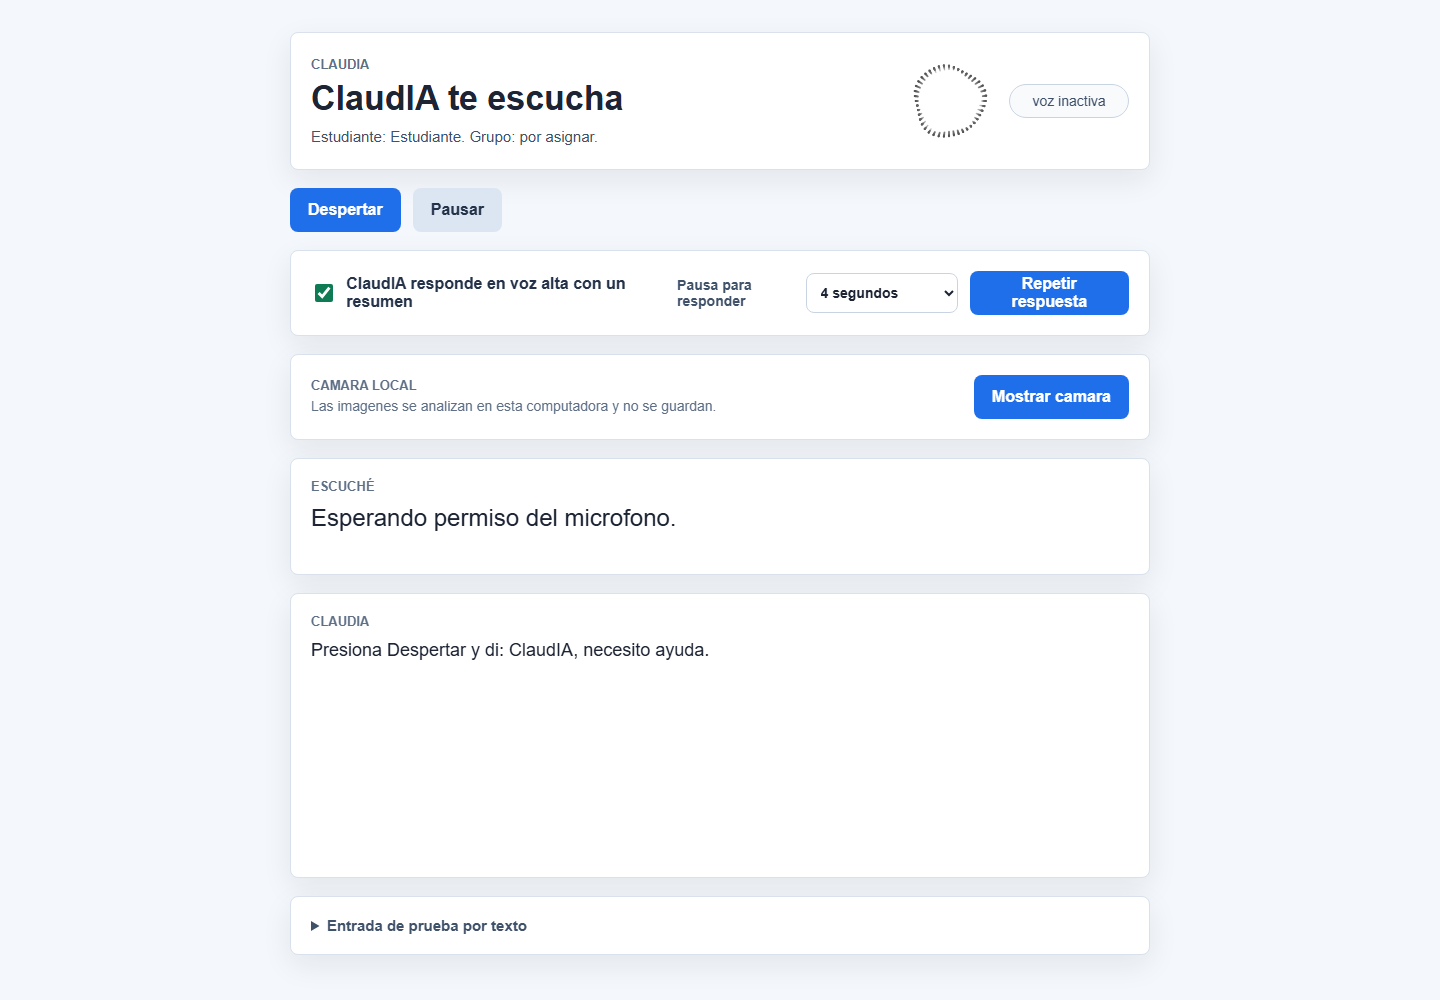
\includegraphics[width=\linewidth,height=2.55in,keepaspectratio]{assets/claudia_web_ui.png}
\end{minipage}\hfill
\begin{minipage}[t]{0.48\textwidth}
\centering
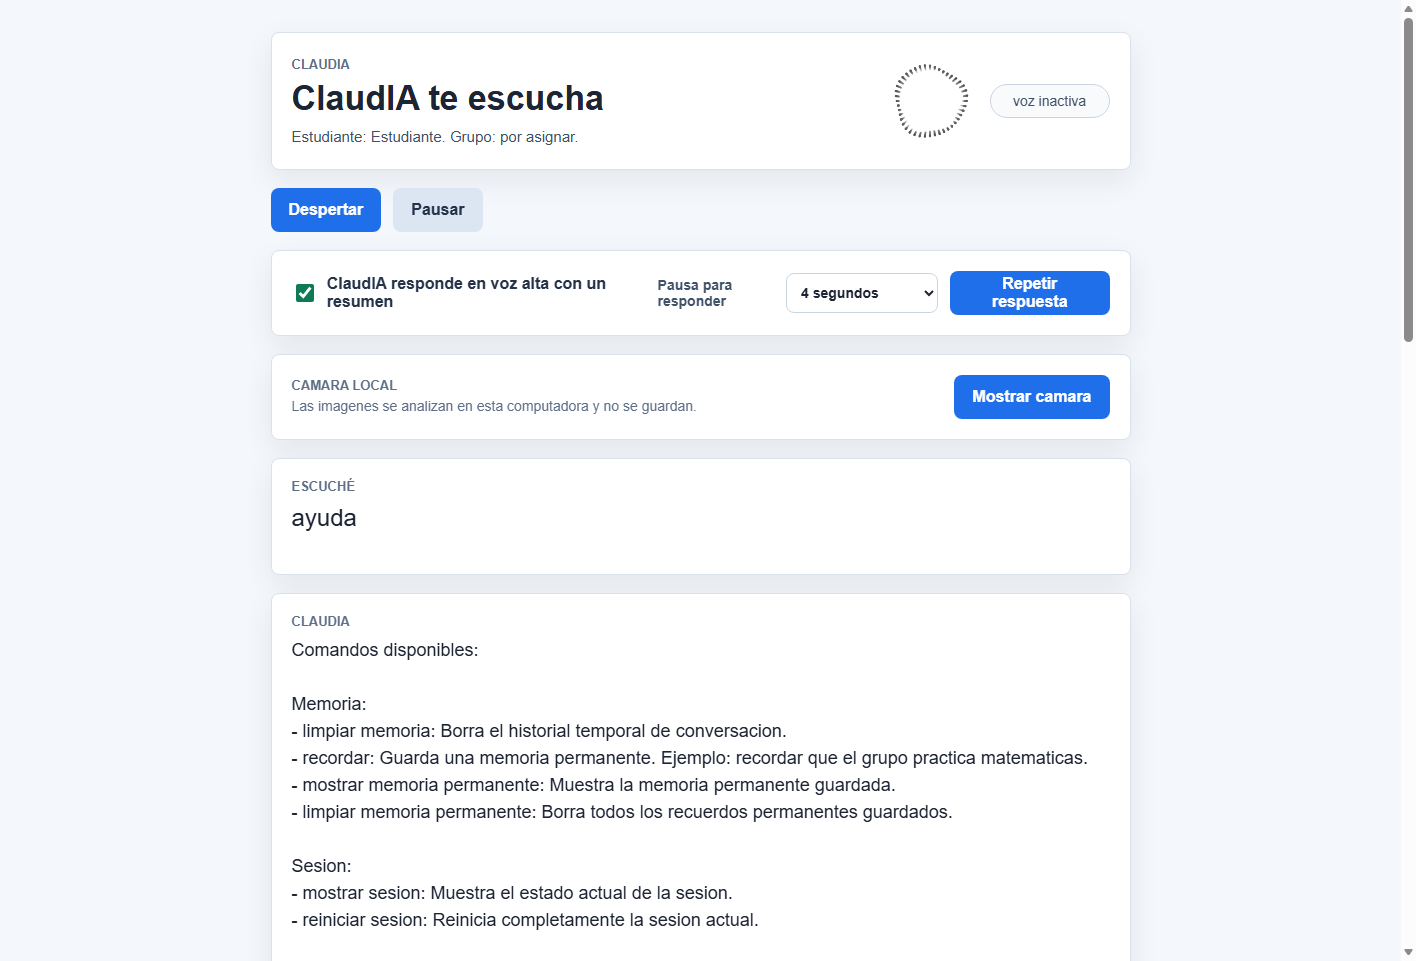
\includegraphics[width=\linewidth,height=2.55in,keepaspectratio]{assets/claudia_web_help.png}
\end{minipage}
\end{center}

\ManualCaption{Figuras 1 y 2. Interfaz local de ClaudIA en espera y respuesta del comando \texttt{ayuda}. La estación muestra el contexto escolar, los controles de escucha, la pausa configurable, la cámara local y las áreas separadas de transcripción y respuesta.}

Las capturas evidencian una interfaz distinta de un chatbot genérico. La pantalla hace visible quién usa la estación, cuándo escucha y cuándo se activa la cámara. Además, separa la transcripción de la respuesta y permite una entrada de prueba por texto para verificar el flujo sin micrófono.

\begin{table}[H]
\centering
\caption{Condiciones de la ejecución documentada}
\begin{tabularx}{\textwidth}{@{}>{\bfseries}p{1.55in}X@{}}
\toprule
Elemento & Resultado observado \\
\midrule
Repositorio & \texttt{ClaudIA-repo}, rama \texttt{master}, commit \texttt{29db70a} \\
Comando & \texttt{npm start} \\
Servicio & \texttt{WebVoiceInterface}, sin errores de inicio \\
Proveedor de IA & DeepSeek configurado como principal \\
Cámara & Análisis local; no conserva video por defecto \\
Evidencia visual & Texto autocontenido y legible en la interfaz \\
\bottomrule
\end{tabularx}
\end{table}

\clearpage

% ---------------------------------------------------------------------------
% PÁGINA 28 - PRUEBAS AUTOMATIZADAS
% ---------------------------------------------------------------------------
\Section{Pruebas automatizadas y operación local}

La validación técnica ejecutó el comando \texttt{npm test}. El resultado fue de 92 pruebas aprobadas, ninguna fallida, cancelada u omitida. La ejecución se realizó sobre el commit \texttt{29db70a} y no consumió tokens de IA porque los proveedores se sustituyeron por clientes simulados.

\begin{center}
\begin{tabularx}{0.88\textwidth}{@{}>{\bfseries}p{1.55in}X@{}}
\toprule
Resultado & Valor reportado \\
\midrule
Pruebas totales & 92 \\
Pruebas aprobadas & 92 \\
Pruebas fallidas & 0 \\
Canceladas / omitidas & 0 / 0 \\
\bottomrule
\end{tabularx}
\end{center}

\Subsection{Cobertura funcional}
\begin{table}[H]
\centering
\caption{Áreas cubiertas por la batería automatizada}
\begin{tabularx}{\textwidth}{@{}>{\raggedright\arraybackslash}p{1.60in}>{\raggedright\arraybackslash}X@{}}
\toprule
\textbf{Área} & \textbf{Comportamiento comprobado} \\
\midrule
Núcleo y comandos & Eventos, rutas, alias, sugerencias y estados válidos \\
Memoria y sesión & Memoria persistente, reinicio y separación por estudiante o grupo \\
Educación y tutoría & Lecciones, progreso, ejercicios, respuestas y pistas \\
Documentos & Lectura permitida, extensiones válidas y rechazo de rutas externas \\
Voz web & Activación, transcripción, pausa de locución y voz mexicana \\
Visión & Estado, errores controlados y reutilización del análisis \\
Proveedores de IA & DeepSeek principal, respaldo y operación sin clave \\
Clase y presentaciones & Contexto docente, recuperación de la clase y generación LaTeX \\
Registro & Mensajes, respuestas y evidencia mínima de interacción \\
\bottomrule
\end{tabularx}
\end{table}

La reproducción requiere ejecutar \texttt{npm install}, \texttt{npm run setup},
\texttt{npm run doctor}, \texttt{npm test} y \texttt{npm start} en ese orden.

La efectividad pedagógica se comprobará en el piloto; la prueba técnica confirma la integración del software.

\clearpage

% ---------------------------------------------------------------------------
% PÁGINA 29 - ANEXO TÉCNICO DE SOFTWARE
% ---------------------------------------------------------------------------
\Section{Anexo C. Arquitectura del repositorio}

El punto de composición \texttt{createClaudiaSystem} construye una instancia de la arquitectura de ClaudIA. Los servicios se inyectan en lugar de importarse de forma global, lo que permite probarlos por separado.

\begin{lstlisting}
export function createClaudiaSystem({ loggerEnabled = true } = {}) {
  const logger = new Logger({ enabled: loggerEnabled });
  const eventBus = new EventBus({ logger });
  const sessionManager = new SessionManager({
    logger,
    profile: claudiaProfile,
  });
  const aiService = new LLMService({ logger, eventBus });
  const visionManager = new VisionManager({
    bridge: visionPythonBridge,
    logger,
  });
  const claudiaCore = new ClaudiaCore({
    eventBus, conversationManager, commandRouter,
    commandInterpreter, stateMachine, logger,
  });
  claudiaCore.registerEvents();
  return { logger, eventBus, sessionManager, aiService,
           visionManager, claudiaCore };
}
\end{lstlisting}

\begin{table}[H]
\centering
\caption{Módulos principales y responsabilidad}
\begin{tabularx}{\textwidth}{@{}>{\raggedright\arraybackslash}p{1.35in}>{\raggedright\arraybackslash}X@{}}
\toprule
\textbf{Módulo} & \textbf{Responsabilidad} \\
\midrule
\texttt{core} & Eventos, estado, ruteo y respuesta principal \\
\texttt{commands} & Interpretación y ejecución de órdenes \\
\texttt{memory} & Sesión temporal y memoria permanente \\
\texttt{education} & Catálogo, lecciones y progreso \\
\texttt{tutor} & Explicación gradual, práctica y pistas \\
\texttt{documents} & Lectura de materiales internos de apoyo \\
\texttt{voice} & Entrada por voz y procesamiento de transcripciones \\
\texttt{vision} & Presencia local mediante puente Python \\
\texttt{ai} & Proveedor DeepSeek y respaldo OpenAI \\
\texttt{classroom} & Contexto de docente, grupo y clase \\
\texttt{presentations} & Materiales LaTeX a partir de una solicitud explícita \\
\bottomrule
\end{tabularx}
\end{table}

La arquitectura conserva la regla de que la interfaz no ejecuta lógica pedagógica ni llama directamente al proveedor. La voz se transforma en una intención y pasa por los mismos comandos que la entrada textual.

\clearpage

% ---------------------------------------------------------------------------
% PÁGINA 30 - ANEXO DE INTERFACES Y PROVEEDOR
% ---------------------------------------------------------------------------
\Section{Anexo D. Interfaces y proveedor de IA}

La interfaz HTTP expone un estado de salud, activación y desactivación de voz, recepción de transcripciones, mensajes de prueba, análisis de cuadros de cámara y un canal de eventos para actualizar la pantalla sin recargarla.

\begin{table}[H]
\centering
\caption{Interfaces locales principales}
\begin{tabularx}{\textwidth}{@{}>{\ttfamily\small}p{1.63in}>{\raggedright\arraybackslash}X@{}}
\toprule
\normalfont\textbf{Ruta} & \textbf{Función} \\
\midrule
/health & Estado del servicio, sesión y proveedor \\
/api/voice/enable & Habilita la entrada por voz \\
/api/voice/disable & Pausa la entrada por voz \\
/api/voice/transcript & Procesa una transcripción recibida \\
/api/message & Envía una entrada de prueba por texto \\
/api/vision/frame & Analiza un cuadro local de cámara \\
/api/voice/events & Transmite cambios de estado a la interfaz \\
\bottomrule
\end{tabularx}
\end{table}

El servicio de lenguaje selecciona DeepSeek como proveedor principal cuando la clave está presente. OpenAI funciona como respaldo únicamente si se configura. Cuando no existe proveedor, ClaudIA inicia en modo local y comunica la limitación en lugar de simular una respuesta académica.

\begin{lstlisting}
const PROVIDER_NAMES = Object.freeze(["deepseek", "openai"]);

async generateResponse(messages, options = {}) {
  const attempts = [...new Set(
    [this.primaryProvider, this.fallbackProvider].filter(Boolean)
  )];
  if (attempts.length === 0) {
    return "La inteligencia artificial todavía no está configurada...";
  }
  for (const providerName of attempts) {
    const response = await provider.client.chat.completions.create({
      model: provider.model,
      messages,
      temperature: options.temperature ?? 0.4,
    });
    return extractContent(response);
  }
}
\end{lstlisting}

\Subsection{Privacidad de las interfaces}
La cámara trabaja de forma local y no guarda la imagen por defecto. La clave de IA se mantiene en variables de entorno y no se incluye en Git. Los registros de interacción se almacenan localmente en formato JSONL para revisar el comportamiento, con exclusión de audio y video.

\clearpage

% ---------------------------------------------------------------------------
% PÁGINA 31 - MATRIZ DE TRAZABILIDAD
% ---------------------------------------------------------------------------
\Section{Anexo E. Matriz de verificación y alcance}

La matriz distingue la evidencia disponible de los aspectos que todavía deben validarse.

\begin{table}[H]
\centering
\caption{Criterios, evidencia y estado de validación}
\footnotesize
\begin{tabularx}{\textwidth}{@{}>{\raggedright\arraybackslash}p{1.45in}>{\raggedright\arraybackslash}X>{\raggedright\arraybackslash}p{1.15in}@{}}
\toprule
\textbf{Criterio} & \textbf{Evidencia disponible} & \textbf{Estado} \\
\midrule
Necesidad educativa & Encuesta a 122 estudiantes: organización y comprensión concentran 74.6\% & Documentada \\
Integración funcional & Núcleo, comandos, memoria, tutor, voz y visión conectados & Probada en laboratorio \\
Calidad técnica & 92 pruebas automatizadas aprobadas, sin fallos & Verificada \\
Interacción & Interfaz local con voz, pausa, cámara y entrada de prueba & Demostrada \\
Riesgos de privacidad & Cámara local sin video por defecto y controles por roles & Diseño definido \\
Efectividad pedagógica & Línea base diagnóstica; piloto aún pendiente & No demostrada \\
Propiedad intelectual & Ruta institucional de autoría y transferencia & Por formalizar \\
\bottomrule
\end{tabularx}
\end{table}

\Subsection{Consistencia de alcance}
ClaudIA no reconoce rostros, no interpreta cuadernos, no diagnostica condiciones de salud y no califica automáticamente. El modelo se usa como mediador y sus respuestas requieren verificación humana.

\clearpage

% ---------------------------------------------------------------------------
% REFERENCIAS
% ---------------------------------------------------------------------------
\begin{thebibliography}{99}
\fontsize{8.2}{10.2}\selectfont
\setlength{\itemsep}{2pt}

\bibitem{cast2024}
CAST. (2024). \textit{Universal Design for Learning Guidelines version 3.0}. \url{https://udlguidelines.cast.org/}

\bibitem{dgeti2026}
Dirección General de Educación Tecnológica Industrial y de Servicios. (2026). \textit{XXIX Concurso Nacional de Prototipos y Proyectos de Emprendimiento 2027}. Secretaría de Educación Pública. \url{https://dgeti.sep.gob.mx/sigepe/}

\bibitem{eef2018}
Education Endowment Foundation. (2018). \textit{Metacognition and self-regulated learning: Guidance report}. \url{https://educationendowmentfoundation.org.uk/education-evidence/guidance-reports/metacognition}

\bibitem{eef2021}
Collin, J., y Quigley, A. (2021). \textit{Teacher feedback to improve pupil learning: Guidance report}. Education Endowment Foundation. \url{https://educationendowmentfoundation.org.uk/education-evidence/guidance-reports/feedback}

\bibitem{gubareva2020}
Gubareva, R., y Lopes, R. P. (2020). Virtual assistants for learning: A systematic literature review. \textit{Proceedings of the 12th International Conference on Computer Supported Education, 1}, 97-103. \url{https://doi.org/10.5220/0009417600970103}

\bibitem{inegi2026}
Instituto Nacional de Estadística y Geografía e Instituto Federal de Telecomunicaciones. (2026). \textit{Encuesta Nacional sobre Disponibilidad y Uso de Tecnologías de la Información en los Hogares 2025: reporte de resultados}. \url{https://www.inegi.org.mx/programas/endutih/2025/}

\bibitem{licona2024}
Licona Quiterio, O. (2024). IA y educación en México: entre oportunidades y desafíos. \textit{RIESED. Revista Internacional de Estudios sobre Sistemas Educativos, 3}(15), 675-688.

\bibitem{ma2014}
Ma, W., Adesope, O. O., Nesbit, J. C., y Liu, Q. (2014). Intelligent tutoring systems and learning outcomes: A meta-analysis. \textit{Journal of Educational Psychology, 106}(4), 901-918. \url{https://doi.org/10.1037/a0037123}

\bibitem{miao2024}
Miao, F., y Shiohira, K. (2024). \textit{AI competency framework for students}. UNESCO. \url{https://doi.org/10.54675/JKJB9835}

\bibitem{nist2023}
National Institute of Standards and Technology. (2023). \textit{Artificial Intelligence Risk Management Framework (AI RMF 1.0)}. NIST AI 100-1. \url{https://nvlpubs.nist.gov/nistpubs/ai/NIST.AI.100-1.pdf}

\bibitem{nist2024}
National Institute of Standards and Technology. (2024). \textit{Artificial Intelligence Risk Management Framework: Generative Artificial Intelligence Profile}. NIST AI 600-1. \url{https://nvlpubs.nist.gov/nistpubs/ai/NIST.AI.600-1.pdf}

\bibitem{sep2025mccms}
Secretaría de Educación Pública. (2025). Acuerdo número 21/08/25 por el que se establece y regula el Marco Curricular Común de la Educación Media Superior. \textit{Diario Oficial de la Federación}.
 \url{https://dof.gob.mx/nota_detalle.php?codigo=5765757&fecha=15/08/2025&print=true}

\bibitem{unesco2024guide}
Miao, F., y Holmes, W. (2024). \textit{Guía para el uso de IA generativa en educación e investigación}. UNESCO. \url{https://unesdoc.unesco.org/ark:/48223/pf0000389227}

\bibitem{zulfiqar2026}
Zulfiqar, M., e Iqbal, U. (2026). A review of privacy, ethics, and governance challenges associated with camera-based AI surveillance in primary schools. \textit{Cureus Journal of Computer Science, 3}, es44389-026-00146-3. \url{https://doi.org/10.7759/s44389-026-00146-3}

\end{thebibliography}

\clearpage

\Section{Anexo A. Ficha de control del prototipo}
\addcontentsline{toc}{section}{Anexo A. Ficha de control del prototipo}

\begin{tabularx}{\textwidth}{@{}>{\bfseries\color{navy}}p{1.45in}X@{}}
\toprule
Nombre & ClaudIA: Sistema Inteligente de Acompañamiento Didáctico para Grupos DGETI \\
Base técnica & Repositorio ClaudIA, commit \texttt{29db70a} \\
Código provisional & 26-AT625 \\
Entorno de prueba & CETis 20, Ciudad del Carmen, Campeche \\
Fuente diagnóstica & Encuesta SNCyT 2026, 122 registros \\
Pruebas técnicas & 92 de 92 pruebas automatizadas superadas \\
Estado & Integración de software con adaptaciones físicas pendientes \\
\bottomrule
\end{tabularx}

\vspace{12pt}
\Subsection{Declaración de alcance}
ClaudIA se encuentra en fase de prototipo y línea base de investigación. Todavía no se atribuye una mejora comprobable en el aprendizaje; esa valoración requiere el piloto con estudiantes y docentes en condiciones reales de aula.

\clearpage

\Section{Anexo B. Protocolo mínimo de operación}
\addcontentsline{toc}{section}{Anexo B. Protocolo mínimo de operación}

\Subsection{Antes de usar ClaudIA}
\begin{enumerate}
  \item Verificar que la estación esté conectada a la alimentación y a la red autorizada.
  \item Confirmar que la bocina reproduzca el tono de prueba y que el micrófono reciba voz.
  \item Revisar que la cámara tenga el obturador abierto sólo para la actividad prevista.
  \item Iniciar sesión con el rol correspondiente y comprobar el grupo activo.
  \item Cargar la lección, el material o el conjunto de preguntas que se utilizará.
\end{enumerate}

\Subsection{Durante la interacción}
\begin{enumerate}
  \item Activar la estación con una frase o botón visible.
  \item Confirmar el estudiante o grupo activo sin solicitar datos personales innecesarios.
  \item Mantener la cámara limitada a la zona de interacción y sin grabación.
  \item Permitir que ClaudIA formule una pregunta antes de entregar la solución.
  \item Interrumpir la sesión si aparecen datos sensibles o contenidos ajenos a la clase.
\end{enumerate}

\Subsection{Al terminar}
\begin{enumerate}
  \item Cerrar la sesión y desactivar micrófono y cámara.
  \item Revisar el resumen de temas que requieren apoyo docente.
  \item Verificar que no se conserven cuadros de video ni registros de presencia innecesarios.
  \item Registrar incidencias técnicas o pedagógicas relevantes.
  \item Apagar la estación y cubrir la cámara si el equipo permanece en el aula.
\end{enumerate}

\Subsection{Condición de cuidado}
ClaudIA registra señales de práctica y contexto de aprendizaje. No diagnostica condiciones de salud, no asigna calificaciones y no debe usarse para vigilar la conducta fuera de una actividad educativa autorizada.

\end{document}
